\chapter{Analyse et Conception}

\section{Etudes préliminaires}

\subsection{Choix méthodologiques }

Avant de se lancer dans les activités du projet, il convient donc de choisir la méthodologie de gestion de projet et le langage de modélisation à utiliser. 

\subsubsection{Gestion de projet}

	Pour le pilotage de notre projet, il existe des méthodes de gestion de projet. Parmi celles-ci,  nous devons choisir une qui convient le mieux non seulement à notre projet mais également à notre contexte en entreprise. Pour ce faire, nous allons tout d’abord effectuer une comparaison de ces méthodes afin de faire un choix convenable.\\
Alors que les méthodes traditionnelles visent à traiter les différentes phases d’un projet d’une manière séquentielle (que l’on nomme aussi cycle de développement en cascade ou encore cycle en V), le principe des méthodes Agiles est de le découper en sous-parties ou sous-projets autonomes (on parle également de développement itératif) qui forment le projet dans sa globalité. 
Nous allons présenter dans un tableau, une étude comparative de l’approche de gestion de projet entre les méthodes agiles et traditionnelles. \\

% Please add the following required packages to your document preamble:
% \usepackage[table,xcdraw]{xcolor}
% If you use beamer only pass "xcolor=table" option, i.e. \documentclass[xcolor=table]{beamer}
% \usepackage[normalem]{ulem}
% \useunder{\uline}{\ul}{}
\begin{table}[H]
\centering
	\caption{Comparaison des approches de gestion de projet}
\begin{tabular}{|l|l|l|}
\hline
\textbf{Thème}                       & \textbf{Approche traditionnelle}                                                                                                                                                               & \cellcolor[HTML]{EFEFEF}Approche agile                                                                                                                                                                                       \\ \hline
{\color[HTML]{333333} Cycle de vie}  & {\color[HTML]{333333} \begin{tabular}[c]{@{}l@{}}En cascade ou en V, phases\\ séquentielles\end{tabular}}                                                                                      & Itérative et incrémentale                                                                                                                                                                                                    \\ \hline
{\color[HTML]{333333} Planification} & {\color[HTML]{333333} \begin{tabular}[c]{@{}l@{}}Prédictive: produite en \\ quantité importante comme \\ support de communication, \\ de validation et de \\ contractualisation.\end{tabular}} & \begin{tabular}[c]{@{}l@{}}Adaptative: réduite au strict \\ nécessaire au profil \\ d’incréments fonctionnels \\ opérationnels pour le \\ feedback du client\end{tabular}                                                    \\ \hline
Equipe                               & \begin{tabular}[c]{@{}l@{}}Contrôle de qualité à la fin \\ du cycle de développement. \\ Le client découvre le produit \\ fini\end{tabular}                                                    & \begin{tabular}[c]{@{}l@{}}Un contrôle de qualité \\ précoce et permanent au \\ niveau du produit et du \\ processus. Le client \\ visualise les résultats tôt \\ et fréquemment\end{tabular}                                \\ \hline
Qualité                              & \begin{tabular}[c]{@{}l@{}}Une équipe avec des \\ ressources spécialisées, \\ dirigée par un chef de projet\end{tabular}                                                                       & \begin{tabular}[c]{@{}l@{}}Une équipe responsabilisée \\ où l’initiative et la commu- \\ nication sont privilégiées \\ soutenues par le chef de projet\end{tabular}                                                          \\ \hline
Suivi d’avancement                   & \begin{tabular}[c]{@{}l@{}}Mesure de la conformité \\ aux plans initiaux. Analyse \\ des écarts.\end{tabular}                                                                                  & \begin{tabular}[c]{@{}l@{}}Un seul indicateur d’avance- \\ ment: le nombre de fonction-\\ nalités implémentées et le \\ travail restant à faire.\end{tabular}                                                                \\ \hline
Changement                           & \begin{tabular}[c]{@{}l@{}}Résistance voire d'opposition \\ au changement, processus \\ lourd de gestion de \\ changements acceptés\end{tabular}                                               & \begin{tabular}[c]{@{}l@{}}Accueil favorable aux \\ changements\end{tabular}                                                                                                                                                 \\ \hline
Gestion des risques                  & \begin{tabular}[c]{@{}l@{}}Processus distinct, rigoureux \\ de gestion des risques.\end{tabular}                                                                                               & \begin{tabular}[c]{@{}l@{}}Gestion des risques intégrée \\ dans le processus global, avec \\ responsabilisation de chacun \\ dans l’identification et la \\ résolution des risques. Pilotage \\ par les risques\end{tabular} \\ \hline
Mesure du succès                     & \begin{tabular}[c]{@{}l@{}}Respect des engagements \\ initiaux en termes de coût, \\ de budget et ce niveau de qualité\end{tabular}                                                            & \begin{tabular}[c]{@{}l@{}}Satisfaction client par la \\ livraison de valeur ajoutée\end{tabular}                                                                                                                            \\ \hline
\end{tabular}
\end{table}

\textbf{SCRUM: une approche itérative et flexible}\\

\textbf{\textit{→ Qu’est-ce que la méthode Scrum? }}\\ 
	Scrum est un cadre de travail pour le développement, la livraison et la maintenance de produits complexes. Basée sur le manifeste Agile rédigé en 2001 par des experts en développement d’application, la méthode Scrum repose sur une gestion de projet collaborative et un cycle de développement itératif (répété plusieurs fois, de l’idée initiale à une version de plus en plus aboutie), incrémental (progressif, tâches après tâches) et adaptatif. 

\textbf{\textit{→ Pourquoi Scrum? }}\\
	Si l’on développe un produit, les besoins des clients ou de l’employeur ne sont pas figés. Nous pouvons émettre des propositions susceptibles de leur donner de nouvelles idées sur lesquelles rebondir. Cette flexibilité demandée est ce qu’on appelle l’agilité. Finis les cahiers des charges détaillés sous toutes les coutures ! Finie la planification rigide et contraignante !

\textbf{\textit{→ Les piliers de Scrum? }}\\
Elle repose sur 3 piliers: \\
	- la transparence, dans la communication et le suivi,\\
	- l’inspection régulière pour détecter les écarts entre les objectifs et le travail réalisé,\\
	- l’adaptation, pour un ajustement en permanence face aux contraintes.

\textbf{\textit{→ Equipe Scrum? }}\\
	Auto-organisée et pluridisciplinaires et définissant un modèle d’équipe optimisant la flexibilité, la créativité et la productivité, une équipe Scrum comprend: \\
	- Un Product Owner  qui porte la vision du produit à réaliser et travaille en interaction avec l’équipe de développement. Il s’agit généralement d’un expert du domaine métier du projet, \\
	- Development Team (équipe de développement),  qui est chargée de transformer les besoins exprimés par le Product Owner en fonctionnalités utilisables. Elle est pluridisciplinaire et peut donc encapsuler d’autres rôles tels que développeur, architecte logiciel, DBA, analyste fonctionnel, graphiste/ergonome, ingénieur système,\\
	- Un Scrum Master, chargé de promouvoir et supporter Scrum tel que défini dans son Guide. Il a donc un rôle de coach à la fois auprès du Product Owner et auprès de l’équipe de développement. Il doit donc faire preuve de pédagogie. Il est également chargé de s’assurer que l’équipe de développement est pleinement productive.\\
Les équipes Scrum livrent des produits de manière itérative et incrémentale, maximisant ainsi les opportunités de retour d’information. Les livraisons incrémentales d’un produit « Fini » assurent la disponibilité d’une version potentiellement utile du produit fonctionnel.

\textbf{\textit{→ Les avantages de Scrum? }}\\
	\textbf{-} Compréhension du travail et des tâches à accomplir \\
	Appliquer Scrum, c’est subdiviser le projet en plusieurs petites parties réalisables. Cette fragmentation vous oblige à vous demander si toutes les tâches doivent vraiment être effectuées pour mener à bien votre projet, et vous permet d’examiner d’un œil critique leur exécution. Avec votre équipe, vous pouvez ainsi optimiser en continu les étapes qui vous mènent à l’objectif final. \\
	\textbf{-} Transparence et respect  \\
	Scrum exige de la transparence. Les membres de l’équipe doivent savoir ce que les autres accomplissent et le résultat qu’ils peuvent en attendre. Mais chacun peut déterminer comment il accomplit sa tâche. Il n’y a pas de véritable « patron » avec Scrum ; c’est une équipe autopilotée qui collabore en restant autonome.\\
	\textbf{-} Deadlines intégrés  \\
	Comme le projet est subdivisé et que des tâches très spécifiques peuvent être attribuées aux membres de l’équipe, on intègre chaque jour des échéances pour évaluer les avancées des uns et des autres. Cela implique que tout le monde prenne ses responsabilités. Chacun sait quand il doit agir et les membres de l’équipe savent quand ils peuvent attendre quelque chose de lui.\\
	\textbf{-} Visibilité continue \\
Travailler de manière efficace et maline n’est possible que si vous conservez une vue d’ensemble et restez organisé. Pour tout tenir à jour, il faut communiquer ouvertement. C’est vraiment le cœur du processus de travail : pour assurer une bonne réalisation, vous mettez au point avec votre équipe une feuille de route logique. Vous êtes ainsi toujours au fait de la progression du projet. \\
	\textbf{-} Focus et flexibilité \\
Scrum a été conçu non seulement pour améliorer les projets mais aussi pour en accélérer la réalisation. Il importe donc de prévoir une marge de manœuvre pour l’imprévu mais aussi, en fonction des priorités, de pouvoir dire « non » à des demandes ayant peu d’impact sur le succès du projet. Un Scrum Master doit donc surveiller et accompagner le processus. C’est primordial.

\textbf{\textit{→ Ses bénéfices }}\\
Parmi ses bénéfices, l’on a : \\
	- une gestion plus souple, plus intelligente du travail, améliorant l’efficacité des équipes, \\
	- une meilleure visibilité du projet et de son évolution,
une communication interne renforcée, et donc une meilleure cohésion d’équipe, \\
	- le partage des savoirs et la favorisation de l’entraide,
un gain de temps et une meilleure réactivité grâce aux réunions fréquentes et aux insights du client.

\textbf{\textit{→ Dans quels cas utiliser la méthode SCRUM? }}\\
Ce framework, ou cadre de travail, est utile quand : \\
	- L’ensemble d’un projet complexe ne peut être ni anticipé ni planifié entièrement ; \\
	- Son pilotage demande un minimum de flexibilité pour intégrer facilement des changements aux planifications initiales.  \\
Offrant plus de réactivité, la méthode Scrum est plus adaptée que les méthodes traditionnelles pour la gestion des projets web tel que le développement logiciel, car elle traduit et organise les projets de façon simple, transparente et pragmatique. 


\textbf{\textit{→ Quelques contraintes de SCRUM }}\\
	Scrum présente le risque de voir les fonctionnalités s’étendre indéfiniment ou « Scope Creep ». À moins qu’une date de fin soit définie de manière formelle, les parties prenantes peuvent être tentées de rajouter des fonctionnalités. Par ailleurs, si une tâche n'est pas bien définie, l'estimation des coûts et du temps du projet ne sera pas exacte. Dans ce cas, la tâche peut être répartie sur plusieurs sprints. 
	En cas de manque de communication, les membres de l’équipe n’auront pas la possibilité d’apporter des améliorations à la définition des produits. Le guide de Scrum ne définit pas formellement une méthode de gestion des bogues, de réduction de la dette technique. \\ 
	Le fait d’imposer un système de gestion de temps constitue également une contrainte. Tous les événements sont conditionnés dans le temps. Une fois qu'un Sprint commence, sa durée est fixe et ne peut être raccourcie ou allongée. Le Daily Scrum est fixé sur une durée de 15 minutes. Ce mode de fonctionnement ne favorise pas une gestion de temps propre à chaque membre de l’équipe et par conséquent réduit les possibilités d’innovation et d’optimisation.

\subsubsection{L’approche orienté objet }
	L’approche orientée objet considère le logiciel comme une collection d’objets dissociés, identifiés, et définis par des propriétés. Une propriété est soit un attribut, soit une méthode. \\
	La fonctionnalité du logiciel émerge alors de l’interaction entre les différents objets qui le constituent. L’une des particularités de cette approche est qu’elle rapproche les données et leurs traitements associés au sein d’un unique objet. Un objet est caractérisé par plusieurs notions dont : \\
	\textit{L’identité :} L’objet possède une identité, qui permet de le distinguer des autres objets, indépendamment de son état. On construit généralement cette identité grâce à un identifiant découlant naturellement du problème (par exemple une Banque pourra être repéré par un code, un Encaissement par un numéro identifiant ... etc.) \\
	\textit{Les attributs :} Il s’agit des données caractérisant l’objet. Ce sont des variables stockant des informations sur l’état de l’objet. \\
	\textit{Les méthodes :} Les méthodes d’un objet caractérisent son comportement, c’est-à-dire l’ensemble des actions (appelées opérations) que l’objet est à même de réaliser. Ces opérations permettent de faire réagir l’objet aux sollicitations extérieures (ou d’agir sur les autres objets). De plus, les méthodes sont étroitement liées aux attributs, car leurs actions peuvent dépendre des valeurs des attributs, ou bien les modifier. \\ 
	La difficulté de cette modélisation réside dans la création d’une représentation abstraite, sous forme d’objets, d’entités ayant une existence matérielle (Exemple : Banque, Guichet, Caisse ... etc.) ou bien virtuelle (Exemple : Encaissement, Décaissement, Transfert de fonds ... etc.). La Conception Orientée Objet (COO) est la méthode qui conduit à des architectures logicielles fondées sur les objets du système, plutôt que sur la fonction qu’il est censé réaliser. La méthode mise en exergue au niveau de l’approche objet est SCRUM. \\
	Scrum est un cadre de développement logiciel itératif et incrémental (une itération désigne la succession des états de l'enchaînement d’activité, tandis qu’un incrément correspond à une avancée dans les différents stades de développement), centré sur l’architecture (propose différentes perspectives indépendantes et complémentaires, qui permettent de définir un modèle d’architecture) et piloté par les user stories qui illustrent les besoins fonctionnels exprimé par les utilisateurs et donc des cas d’utilisation d’UML (d’où le processus de développement sera centré sur l’utilisateur). C’est un patron de processus pouvant être adapté à une large classe de systèmes logiciels, à différents domaines d’applications, à différents types d’entreprise, à différents niveaux de compétence et à différentes tailles d’entreprise. Scrum gère le processus de développement par deux dimensions. La première représente les principaux enchaînements d’activités qui regroupent les activités selon leur nature. Cette dimension rend compte de l’aspect statique du processus qui s’exprime en termes de composants, de processus, d’activités, d’enchaînements et de travailleurs : \\
		-  Expression des besoins ; \\
		-  Analyse ; \\
		-  Conception ; \\
		-  Implémentation ; \\
		-  Tests. \\
	La seconde dimension représente le temps et montre le déroulement du cycle de vie du processus ; cette dimension rend compte de l’aspect dynamique du processus qui s’exprime en termes de cycle, de phrases, d’itérations et de jalons. 

\subsubsection{UML et MERISE}
	Les différences observées entre ‘approche objet avec UML  et l’approche systématique (fonctionnelle) avec MERISE sont mises en évidence dans l'étude comparative ci-dessous : \\
	- Points commun \\
	L’approche classique et l’approche objet distinguent bien globalement trois grandes étapes dans le processus de conception et de développement d’une solution : l’analyse objet correspond au niveau conceptuel de merise, la conception objet est proche de la modélisation logique et organisationnelle de merise. Et enfin l’implémentation objet correspond à la réalisation dans merise. \\
	Nous allons reprendre chaque grand niveau de représentation du système d’informations  et donner un certain nombre de précisions sur les points communs. \\
Le niveau de l’analyse objet ou le niveau conceptuel : dans les deux approches, la finalité de ces premiers niveaux de description d’un SI est d’appréhender les besoins à satisfaire et donner une description de solutions indépendamment des considérations techniques des niveaux logiciel et physique. Autrement dit les préoccupations traitées sont très proches malgré des concepts pas complètement identiques au niveau conceptuel et au niveau de l’analyse objet. Le niveau conception Objet ou le niveau logique-Organisationnel : ce niveau de description a bien pour finalité dans les deux approches de représenter la solution à implémenter sous l’angle de la logique informatique tant sur la partie des données que sur celle des traitements. \\
Le niveau d'implémentation physique ou opérationnel dans les deux approches la préoccupation est la description physique et opérationnelle des données et traitements. \\
	- Différences \\
	Nous observons les différences entre ces deux approches au niveau des domaines d’application, de la démarche, des données et des traitements puis l’aspect évolution du système. \\
	- Les domaines d’application \\
	Merise a pour vocation de traiter les systèmes d’informations des entreprises, principalement dans le domaine de l’informatique de gestion. Le domaine de l’informatique de gestion se caractérise en général par un grand nombre de données à gérer et à stocker avec des traitements relativement peu complexes. Le domaine privilégié par UML est le domaine de l’informatique technique ou industrielle caractérisé par la gestion de composants physiques du monde réel (Informatisation des automates est représentatif de ce domaine). Dans ce type de domaine les aspects traitements d’états et comportements des objets, prennent le pas sur la gestion des données. En plus de cet atout, UML traite également sans difficulté majeur le domaine tel que l’informatique de gestion. \\
	- La démarche \\
	Avec merise la démarche est structurée en étapes et phases dont l’étude préalable, l’étude détaillée, la réalisation et la mise en œuvre[7]. Il correspond en effet au cycle de vie d’un système d’information. Et l’ensemble des résultats produits à chaque étape constitue le cycle de décision. Merise propose donc une démarche en cascade, c’est-à-dire qu’une étape ne peut être entamée que si l’étape précédente est achevée. Cela nécessite une organisation minutieuse du projet. Dans le cas contraire, l'on pourrait noter quelques blocages ou une lenteur dans le processus de modélisation du système d’information. Avec UML, la démarche est itérative, incrémentale guidée par les besoins des utilisateurs du système, et centrée sur l’architecture logicielle. La démarche itérative permet de mieux comprendre et représenter un système complexe. Le périmètre du système à modéliser est défini par les besoins des utilisateurs (les utilisateurs définissent ce que doit être le système). \\

	- Choix de la méthode d’analyse \\
	Suite à notre étude comparative entre l’approche systémique avec Merise et l’approche Objet avec UML, nous opterons donc pour une méthode d’analyse suivant l’approche Orienté Objet dont UML pour la modélisation, dans l’étude conceptuelle de notre système. Ensuite, vu les circonstances et les délais de notre projet, nous optons pour une démarche itérative, incrémentale guidée par les besoins des utilisateurs du système. De plus, nous souhaiterions organiser nos programmes en rassemblant les données et les traitements en vue de former des entités cohérentes, logiques et stables. Enfin nous aimerions faciliter les éventuelles évolutions et maintenances du système. 
	
	
\section{Analyse du système}

\subsection{Modélisation fonctionnelle }
	La modélisation fonctionnelle est une démarche qui consiste à rechercher et à caractériser les fonctions offertes par un produit pour satisfaire les besoins d’un utilisateur.

\textbf{\textit{→ Diagramme de bête à Corne: }}\\
	C’est un outil d’analyse fonctionnelle  qui permet l’expression du besoin. Dans le lancement d’un projet, il est nécessaire d’expliciter simplement le besoin primaire, c’est-à-dire l’exigence principale. \\
	
	La règle à suivre est de répondre aux trois questions: \\
	- A qui, à quoi le produit rend-t-il service ? à l’élève \\
	- Sur qui, sur quoi agit-il ? Les cours et exercices de mathématiques \\
	- Dans quel but existe-t-il ? 
\begin{figure}[hbtp]
\centering
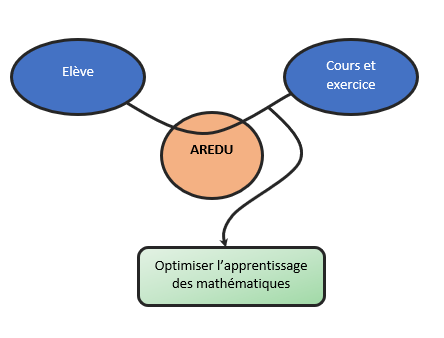
\includegraphics[scale=1]{img/DBaC.png}
\caption{Diagramme de bête à corne}
\end{figure}

\noindent

→ Dans le langage UML, la modélisation fonctionnelle passe par: \\
	- L’identification des acteurs \\
	- L’identification des cas d’utilisation \\
	- Réalisation du diagramme de cas d’utilisation \\
	- Description textuelle et graphique des cas d’utilisation 


\subsubsection{Identification des acteurs}
	Un acteur représente un rôle joué par une entité externe (utilisateur humain, dispositif matériel ou autre système) qui interagit directement avec le système. Dans le cadre de notre application, nous avons pu identifier ces différents acteurs: 
	\begin{itemize}
		\item L’administrateur 
		\item L’enseignant 
		\item L’apprenant
	\end{itemize}
\subsubsection{Identification des cas d’utilisation}
	Il est question ici de décrire une façon d’utiliser le système et d’en décrire les exigences fonctionnelles. Nous avon retenu les cas d’utilisation suivants: 

% Please add the following required packages to your document preamble:
% \usepackage{multirow}
% \usepackage[table,xcdraw]{xcolor}
% If you use beamer only pass "xcolor=table" option, i.e. \documentclass[xcolor=table]{beamer}
%\begin{table}[]
%\begin{tabular}{|l|l|l|}
%\hline
%\textbf{Acteurs}                                           & \textbf{Cas d’utilisation}                                                    & \cellcolor[HTML]{EFEFEF}\textbf{Description}                                                                                                                                                                            \\ \hline
%{\color[HTML]{333333} }                                    & {\color[HTML]{333333} Créer un chapitre}                                      & \begin{tabular}[c]{@{}l@{}}Depuis un fichier externe ou \\ manuellement (par son id, son \\ libellé et sa description) afin \\ de permettre à l'enseignant \\ d'insérer les notions\end{tabular}                        \\ \cline{2-3} 
%{\color[HTML]{333333} }                                    & {\color[HTML]{333333} Editer un chapitre}                                     & \begin{tabular}[c]{@{}l@{}}Afin de modifier le libellé du \\ chapitre\end{tabular}                                                                                                                                      \\ \cline{2-3} 
%{\color[HTML]{333333} }                                    & Editer le contenu d’un chapitre                                               & \begin{tabular}[c]{@{}l@{}}Afin d’apporter des mises à \\ jours sur le chapitre\end{tabular}                                                                                                                            \\ \cline{2-3} 
%{\color[HTML]{333333} }                                    & Consulter liste des chapitres                                                 & \begin{tabular}[c]{@{}l@{}}Afin de connaître tous les \\ chapitres au programme\end{tabular}                                                                                                                            \\ \cline{2-3} 
%{\color[HTML]{333333} }                                    & Consulter contenu du chapitre                                                 & \begin{tabular}[c]{@{}l@{}}Afin d’afficher les données \\ du chapitre concerné\end{tabular}                                                                                                                             \\ \cline{2-3} 
%{\color[HTML]{333333} }                                    & Supprimer des chapitres                                                       & \begin{tabular}[c]{@{}l@{}}Afin de retirer le chapitre \\ au programme\end{tabular}                                                                                                                                     \\ \cline{2-3} 
%{\color[HTML]{333333} }                                    & Créer un compte                                                               & \begin{tabular}[c]{@{}l@{}}Afin de donner la possibilité à\\  un enseignant de se connecter \\ (via son login et son password)\end{tabular}                                                                             \\ \cline{2-3} 
%{\color[HTML]{333333} }                                    & Modifier un compte                                                            & \begin{tabular}[c]{@{}l@{}}Afin de modifier les \\ informations du compte\end{tabular}                                                                                                                                  \\ \cline{2-3} 
%{\color[HTML]{333333} }                                    & Activer un compte                                                             & \begin{tabular}[c]{@{}l@{}}Afin de rendre fonctionnel / non \\ fonctionnel l'état du compte\end{tabular}                                                                                                                \\ \cline{2-3} 
%{\color[HTML]{333333} }                                    & Désactiver un compte                                                          & \begin{tabular}[c]{@{}l@{}}Afin de rendre non fonctionnel \\ l'état du compte\end{tabular}                                                                                                                              \\ \cline{2-3} 
%{\color[HTML]{333333} }                                    & Supprimer un compte                                                           & \begin{tabular}[c]{@{}l@{}}Afin de retirer l’utilisateur \\ du système\end{tabular}                                                                                                                                     \\ \cline{2-3} 
%{\color[HTML]{333333} }                                    & Consulter la liste des comptes                                                & \begin{tabular}[c]{@{}l@{}}Afin de connaître tous les \\ comptes existants dans le \\ système\end{tabular}                                                                                                              \\ \cline{2-3} 
%{\color[HTML]{333333} }                                    & S’authentifier                                                                & \begin{tabular}[c]{@{}l@{}}Afin d'accéder à son profil \\ ou sa page d’accueil\end{tabular}                                                                                                                             \\ \cline{2-3} 
%{\color[HTML]{333333} }                                    & S’inscrire                                                                    & \begin{tabular}[c]{@{}l@{}}Afin de pouvoir s’authentifier, \\ l’utilisateur doit avoir un \\ compte, donc s’inscrire (en \\ renseignant son email, \\ username, password, surname, \\ téléphone et avatar)\end{tabular} \\ \cline{2-3} 
%\multirow{-15}{*}{{\color[HTML]{333333} L’administrateur}} & S’authentifier                                                                & \begin{tabular}[c]{@{}l@{}}Afin d'accéder à son profil \\ ou sa page d’accueil\end{tabular}                                                                                                                             \\ \hline
%                                                           & Créer une leçon                                                               & \begin{tabular}[c]{@{}l@{}}Afin d’y renseigner des notions \\ (en renseignant l’identifiant \\ de la leçon, son libellé et sa \\ description)\end{tabular}                                                              \\ \cline{2-3} 
%                                                           & \begin{tabular}[c]{@{}l@{}}Consulter les leçons \\ d’un chapitre\end{tabular} & \begin{tabular}[c]{@{}l@{}}Afin de connaître toutes les \\ leçons du chapitre\end{tabular}                                                                                                                              \\ \cline{2-3} 
%                                                           & Modifier une leçon                                                            & \begin{tabular}[c]{@{}l@{}}Afin d’apporter des mises \\ à jours à la leçon\end{tabular}                                                                                                                                 \\ \cline{2-3} 
%                                                           & Supprimer une leçon                                                           & \begin{tabular}[c]{@{}l@{}}Afin de la retirer du \\ chapitre\end{tabular}                                                                                                                                               \\ \cline{2-3} 
%                                                           & Consulter contenu de la leçons                                                & \begin{tabular}[c]{@{}l@{}}Afin d’afficher le contenu \\ de la leçon\end{tabular}                                                                                                                                       \\ \cline{2-3} 
%                                                           & Ajouter une notion à une leçon                                                & \begin{tabular}[c]{@{}l@{}}Afin de l’ajouter dans le \\ système (en renseignant \\ l’identifiant de la notion, son \\ libellé, sa description et sa \\ ressource qui est une vidéo)\end{tabular}                        \\ \cline{2-3} 
%                                                           & Modifier une notion                                                           & \begin{tabular}[c]{@{}l@{}}Afin d’y apporter des mises \\ a jours\end{tabular}                                                                                                                                          \\ \cline{2-3} 
%                                                           & Supprimer une notion                                                          & Afin de la retirer de la leçon                                                                                                                                                                                          \\ \cline{2-3} 
%                                                           & Lister les notions                                                            & \begin{tabular}[c]{@{}l@{}}Afin de connaître toutes les \\ notions de la leçon\end{tabular}                                                                                                                             \\ \cline{2-3} 
%                                                           & Créer un exercice                                                             & \begin{tabular}[c]{@{}l@{}}Afin de le référencer à une \\ notion\end{tabular}                                                                                                                                           \\ \cline{2-3} 
%                                                           & Modifier un exercice                                                          & \begin{tabular}[c]{@{}l@{}}Afin d’y apporter des mises \\ a jours\end{tabular}                                                                                                                                          \\ \cline{2-3} 
%                                                           & Supprimer un exercice                                                         & Afin de le retirer du système                                                                                                                                                                                           \\ \cline{2-3} 
%                                                           & Lister  les exercices                                                         & \begin{tabular}[c]{@{}l@{}}Afin de s'assurer que chaque \\ exercice est associé à une \\ notion\end{tabular}                                                                                                            \\ \cline{2-3} 
%                                                           & Créer un evaluation                                                           & Afin de l’assimiler à un chapitre                                                                                                                                                                                       \\ \cline{2-3} 
%                                                           & Modifier une évaluation                                                       & \begin{tabular}[c]{@{}l@{}}Afin d’y apporter des \\ mises a jour\end{tabular}                                                                                                                                           \\ \cline{2-3} 
%                                                           & Supprimer une évaluation                                                      & Afin de la retirer du système                                                                                                                                                                                           \\ \cline{2-3} 
%\multirow{-17}{*}{L’enseignant}                            & Modifier son profil                                                           & \begin{tabular}[c]{@{}l@{}}Afin d’y apporter des mises \\ a jours\end{tabular}                                                                                                                                          \\ \hline
%                                                           & S’authentifier                                                                & \begin{tabular}[c]{@{}l@{}}Afin d'accéder à son profil ou \\ sa page d’accueil\end{tabular}                                                                                                                             \\ \cline{2-3} 
%                                                           & Lire une notion                                                               & \begin{tabular}[c]{@{}l@{}}Afin de comprendre de quoi \\ il s’agit\end{tabular}                                                                                                                                         \\ \cline{2-3} 
%                                                           & Lire un exercice                                                              & Afin de mieux le comprendre                                                                                                                                                                                             \\ \cline{2-3} 
%                                                           & Traiter un exercice                                                           & \begin{tabular}[c]{@{}l@{}}Afin d’appliquer la notion \\ apprise et de voir si on l’a \\ comprise\end{tabular}                                                                                                          \\ \cline{2-3} 
%                                                           & Soumettre un exercice                                                         & Afin d’avoir une correction                                                                                                                                                                                             \\ \cline{2-3} 
%                                                           & Lire une évaluation                                                           & Afin de mieux la comprendre                                                                                                                                                                                             \\ \cline{2-3} 
%                                                           & Traiter une évaluation                                                        & \begin{tabular}[c]{@{}l@{}}Afin de voir si on a compris \\ le chapitre\end{tabular}                                                                                                                                     \\ \cline{2-3} 
%                                                           & Soumettre une évaluation                                                      & Afin d’avoir une correction                                                                                                                                                                                             \\ \cline{2-3} 
%\multirow{-9}{*}{L’apprenant}                              & Modifier son profil                                                           & \begin{tabular}[c]{@{}l@{}}Afin d’y apporter des mises \\ a jours\end{tabular}                                                                                                                                          \\ \hline
%\end{tabular}
%\end{table}

\begin{figure}[hbtp]
\caption{•}
\centering
%\includegraphics[scale=1]{img/tduc1.PNG}
\end{figure}

\begin{figure}[hbtp]
\caption{•}
\centering
%\includegraphics[scale=1]{img/tduce.PNG}
\end{figure}

\end{figure}

\begin{figure}[hbtp]
\caption{•}
\centering
%\includegraphics[scale=1]{img/tducap.PNG} 
\end{figure}

\subsubsection{Réalisation du diagramme de cas d’utilisation}
	Les cas d’utilisation sont représentés dans un diagramme nommé diagramme des cas d’utilisation. Ce diagramme UML est utilisé afin de donner une vision globale du comportement fonctionnel d’un système logiciel; il est utile pour des présentations auprès de la direction ou des acteurs d’un projet. 
	
\noindent

Un cas d’utilisation (use case) décrit une interaction entre un acteur et le système produisant un résultat particulier. Il modélise un service rendu par le système. Pour chaque acteur identifié précédemment on associe les cas d’utilisation qui lui correspondent. \\
	Les différents diagrammes de cas d’utilisation que nous ressortons sont les suivantes : 
	
\textbf{→ Gestion des comptes}
	\begin{figure}[H]
		\centering
%		\includegraphics[scale=0.6]{img/Diagramme usecase gestion compte.png}
	\caption{Diagramme cas d'utilisation "gestion compte"}
	\end{figure}

\textbf{→ Gestion des chapitres}
	\begin{figure}[H]
	\centering
%	\includegraphics[scale=0.7]{img/Diagramme usecase gestion chapitre.png}
	\caption{Diagramme usecase gestion chapitre}
	\end{figure}
	
\textbf{→ Gestion des leçons }
	\begin{figure}[H]
	\centering
%	\includegraphics[scale=0.5]{img/Diagramme sequence modifier contenu leçon.png}
	\caption{Diagramme sequence modifier contenu leçon}
	\end{figure}
	
\textbf{→ Gestion des notions} 
%	\begin{figure}[hbtp]
%	\caption{Diagramme usecase gestion leçons}
%	\centering
%	\includegraphics[scale=1]{img/Diagramme usecase gestion leçons.png}
%	\end{figure}
%	
\textbf{→ Gestion des exercices}
	\begin{figure}[H]
	\centering
	\includegraphics[scale=1]{img/Diagramme usecase gestion exercice.png}
	\caption{Diagramme usecase gestion exercice}
	\end{figure}

\textbf{→ Gestion des évaluations} 	
	\begin{figure}[H]
	\centering
	\includegraphics[scale=1]{img/Diagramme usecase gestion evaluation.png}
	\caption{Diagramme usecase gestion evaluation}
	\end{figure}
	
\textbf{→ Gestion des tests}
	\begin{figure}[H]
	\caption{Diagramme usecase gestion tests}
	\centering
	\includegraphics[scale=1]{img/Diagramme usecase gestion tests.png}
	\end{figure}
	
En ce qui concerne la vision globale du système, nous avons : \\
%\begin{figure}[H]
%\centering
%\includegraphics[scale=0.5]{img/Diagramme global usecase.png}
%\caption{Diagramme global cas d'utilisation}
%\end{figure}

\begin{figure}[H]
\centering
\includegraphics[scale=0.5]{img/Diagramme global usecase.png}
\caption{Diagramme global usecase}
\end{figure}


\subsubsection{Description textuelle et graphique de quelques cas d’utilisation}
	Nous allons désormais parler de l’interaction entre les acteurs et le système: il s’agira de décrire la chronologie des actions qui devront être réalisées par les acteurs et par le système lui-même. On parle d’ailleurs de scénaris. La description d’un cas d’utilisation permet de: \\
	- Clarifier le déroulement de la fonctionnalité, \\
	- Décrire la chronologie des actions qui devront être réalisées, \\
	- Identifier les parties redondantes pour en déduire des cas d’utilisation plus précises qui seront utilisées par inclusion, extension ou généralisation/spécialisation, \\
	- Indiquer d’éventuelles contraintes déjà connues et dont les développeurs vont devoir tenir compte lors de la réalisation du logiciel. \\
	Nous les effectuerons leur représentation graphique avec les diagrammes de séquence et d’activité. 
	
\paragraph{Diagrammes de séquence} ~~\\
	Le diagramme de séquence montre les interactions entre les utilisateurs et le système vue de l’extérieur du système au moyen d’interface homme-machine. 
Les diagrammes de séquence peuvent constituer des références utiles pour les entreprises et d'autres organisations. L’on réalise un diagramme de séquence pour :
\begin{itemize}
	\item Représenter les détails d'un cas d'utilisation UML
	\item Modéliser le déroulement logique d'une procédure, fonction ou opération complexe
	\item Voir comment les objets et les composants interagissent entre eux pour effectuer un processus.
	\item Schématiser et comprendre le fonctionnement détaillé d'un scénario existant ou à venir
\end{itemize}

Les diagrammes de séquence effectués ici sont les suivants: \\
→ Cas d’utilisation S’authentifier \\
\textbf{But:} Permet à l’utilisateur de se connecter au système \\
\textbf{Acteurs:} administrateur, enseignant, apprenant \\
\textbf{Pré-condition:} l’utilisateur doit avoir un compte \\
\textbf{Scénario nominal:}  \\
L’acteur accède à la page de connexion \\
L’acteur rentre ses informations et valide \\
Le système vérifie si les informations reçues sont exactes \\
Le système connecte l’acteur et affiche la page d’accueil \\
\textbf{Alternative:}  \\
        Erreur de connexion (Les données entrées par l’utilisateur n’existent pas): login ou mot de passe non valide \\
Le système affiche un message d’erreur correspondant au problème \\
	        Le scénario reprend au point 2 \\
\textbf{Post-condition} \\
 - Acteur connecté 
 
 \begin{figure}[hbtp]
 \centering
 \includegraphics[scale=1]{img/Diagramme sequence authentification.png}
 \caption{Diagramme sequence authentification}
 \end{figure}
 

→ Cas d’utilisation Créer un chapitre
But: Ajouter un chapitre dans le système 
Acteurs: administrateur
Pré-condition: administrateur connecté
Scénario nominal 
L’administrateur clique sur ajouter un chapitre
Le système affiche la page d’ajout
L’acteur rempli le formulaire et le soumet
Le système vérifie si les informations émises
Le système enregistre le chapitre, puis fais la mises à jour et redirige vers la liste des chapitres
Scénario alternatif  
Champ(s) correcte(s) ou obligatoire(s) vide(s) 
	           L'enchaînement démarre au point 4
Le système sélectionne les champs concernés
	           Le scénario reprend au point 3
Chapitre existant
           L'enchaînement démarre au point 4
Post-condition 
Chapitre créé


\section{Conception générale}
